Рассмотрим первый пример. 

Если $k = 1$, то телепортаций не происходит.

Если $k=2$, то гонка происходит следующим образом. На рисунках показаны моменты, когда дроны оказываются в воротах и происходит телепортация.

\medskip
\begin{center}
\begin{tabular}{cc}
\renewcommand{\arraystretch}{2}
%>{\centering}p{5cm}
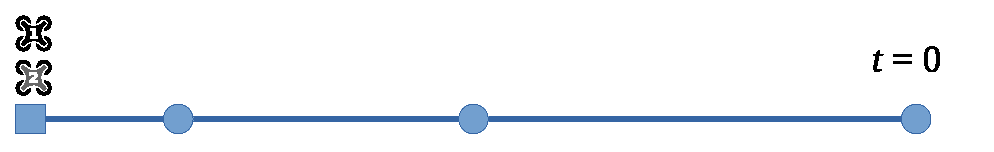
\includegraphics[scale=0.7]{sample-2-01.eps}\\[0.8cm]

\includegraphics[scale=0.7]{sample-2-02.eps}\\[0.3cm]
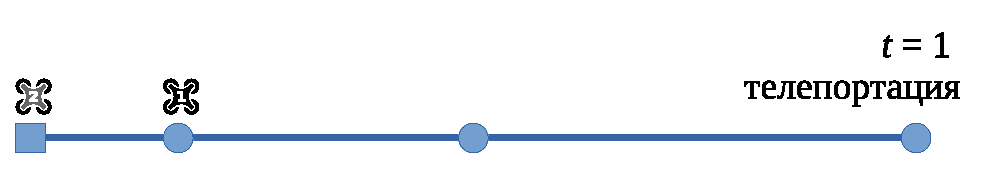
\includegraphics[scale=0.7]{sample-2-03.eps}&{1 телепортация}\\[0.8cm]

\includegraphics[scale=0.7]{sample-2-04.eps}\\[0.3cm]
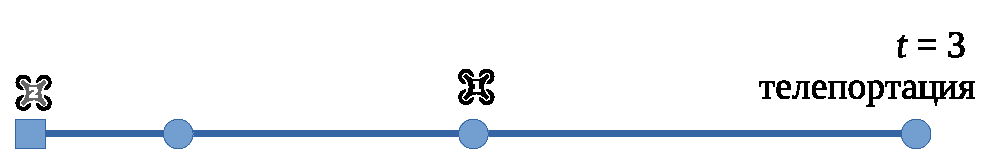
\includegraphics[scale=0.7]{sample-2-05.eps}&{+1 телепортация, итого 2}\\[0.8cm]
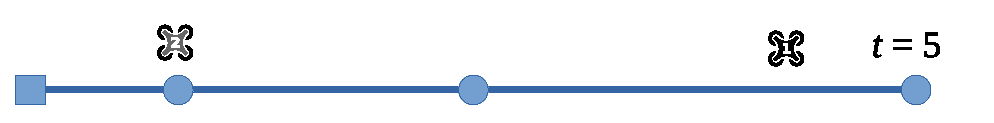
\includegraphics[scale=0.7]{sample-2-06.eps}\\[0.3cm]
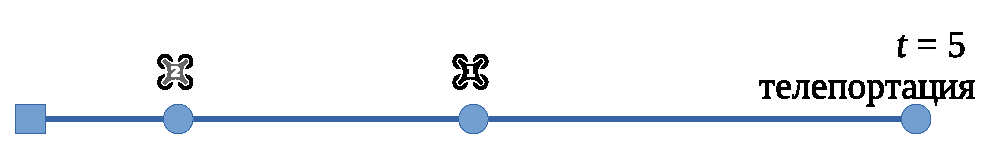
\includegraphics[scale=0.7]{sample-2-07.eps}&{+1 телепортация, итого 3}\\[0.8cm]
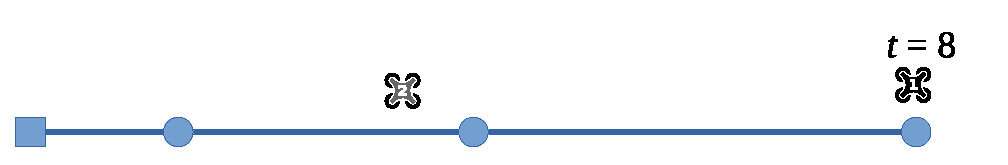
\includegraphics[scale=0.7]{sample-2-08.eps}&дрон 1 финишировал\\[0.3cm]
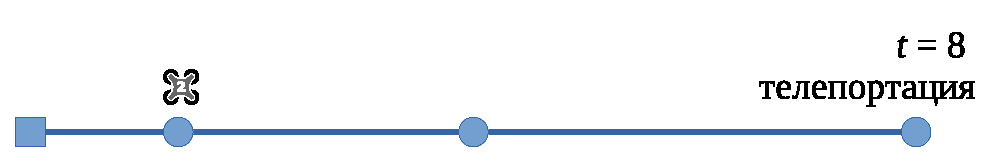
\includegraphics[scale=0.7]{sample-2-09.eps}&{+1 телепортация, итого 4}\\[0.8cm]
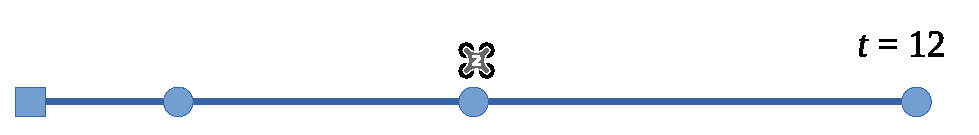
\includegraphics[scale=0.7]{sample-2-10.eps}\\[0.8cm]
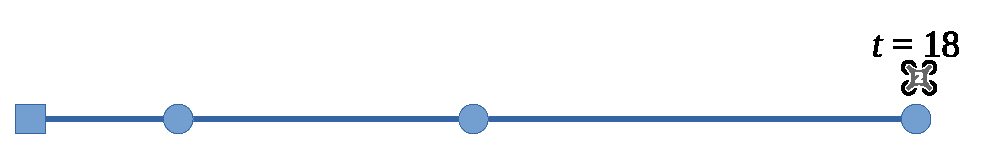
\includegraphics[scale=0.7]{sample-2-11.eps}&дрон 2 финишировал\\
\end{tabular}
\end{center}

Если $k=3$, то гонка происходит следующим образом. На рисунках показаны моменты, когда дроны оказываются в воротах и происходит телепортация.


\begin{center}
\begin{tabular}{cc}
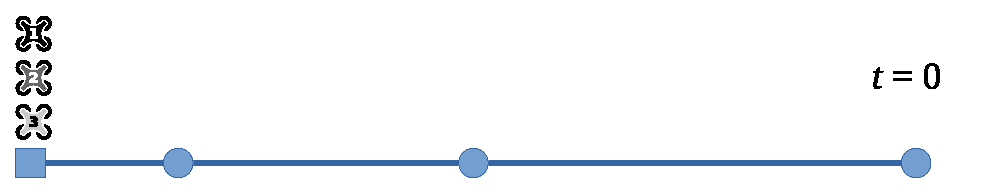
\includegraphics[scale=0.5]{sample-3-01.eps}\\[0.5cm]

\includegraphics[scale=0.5]{sample-3-02.eps}&
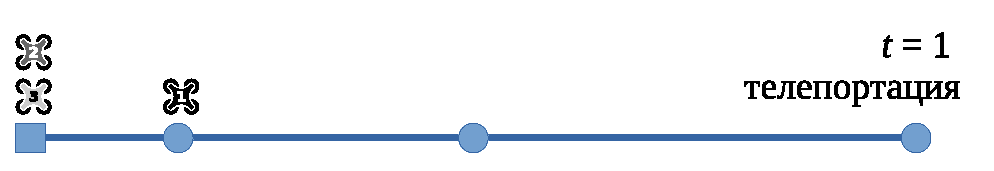
\includegraphics[scale=0.5]{sample-3-03.eps}\\
&2 телепортации\\[0.5cm]

\includegraphics[scale=0.5]{sample-3-04.eps}&
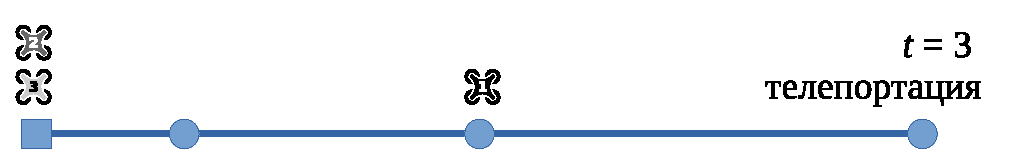
\includegraphics[scale=0.5]{sample-3-05.eps}\\
&+2 телепортации, итого 4\\[0.5cm]

\includegraphics[scale=0.5]{sample-3-06.eps}&
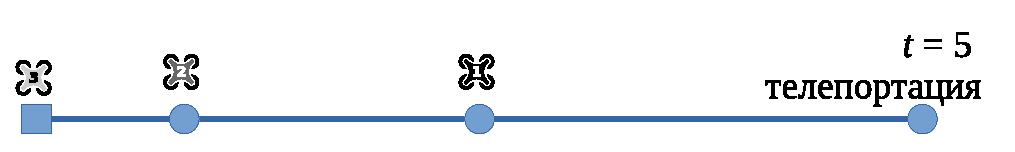
\includegraphics[scale=0.5]{sample-3-07.eps}\\
&+2 телепортации, итого 6\\[0.5cm]
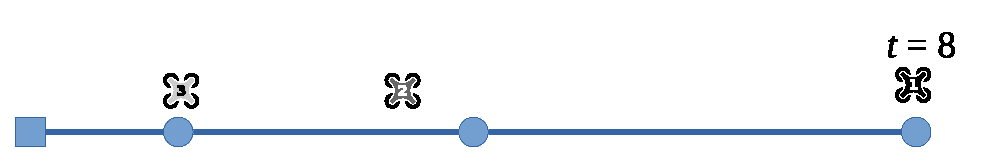
\includegraphics[scale=0.5]{sample-3-08.eps}&
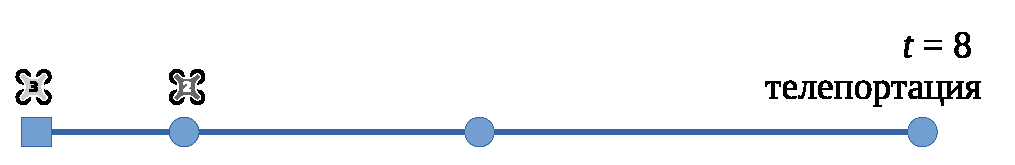
\includegraphics[scale=0.5]{sample-3-09.eps}\\
дрон 1 финишировал &+2 телепортации, итого 8\\[0.5cm]
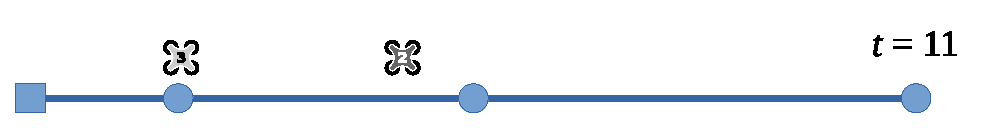
\includegraphics[scale=0.5]{sample-3-10.eps}&
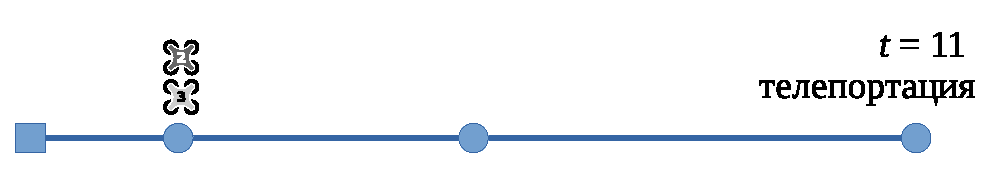
\includegraphics[scale=0.5]{sample-3-11.eps}\\
&+1 телепортация, итого 9\\[0.5cm]
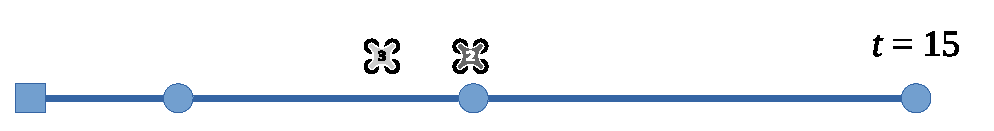
\includegraphics[scale=0.5]{sample-3-12.eps}&
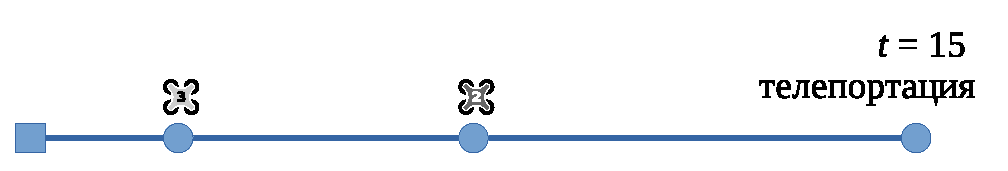
\includegraphics[scale=0.5]{sample-3-13.eps}\\
&+1 телепортация, итого 10\\[0.5cm]
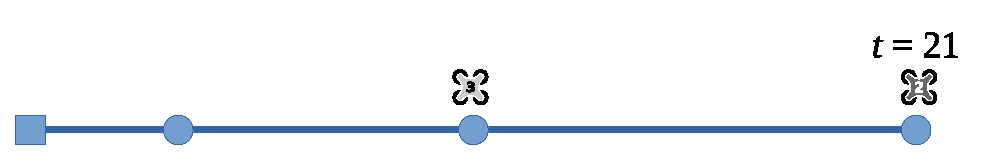
\includegraphics[scale=0.5]{sample-3-14.eps}&
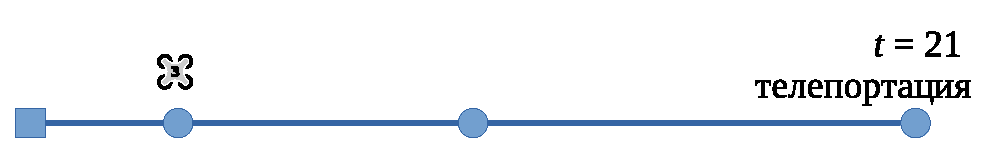
\includegraphics[scale=0.5]{sample-3-15.eps}\\
дрон 2 финишировал&+1 телепортация, итого 11\\[0.5cm]
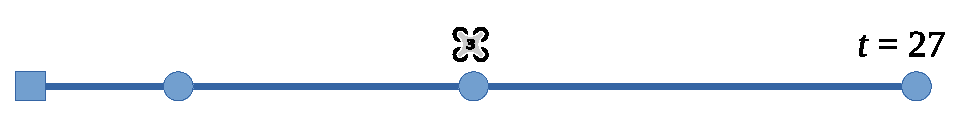
\includegraphics[scale=0.5]{sample-3-16.eps}&
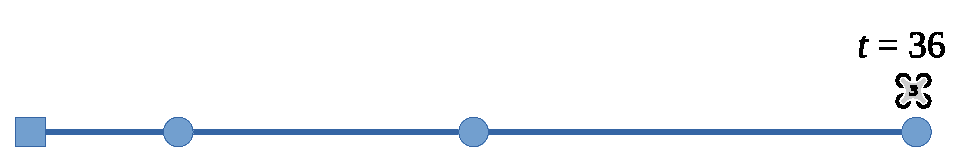
\includegraphics[scale=0.5]{sample-3-17.eps}\\
&дрон 3 финишировал\\
\end{tabular}
\end{center}


